\documentclass{beamer}
\setbeamertemplate{navigation symbols}{}
\usepackage{comment}

\setbeamercolor{frametitle}{fg=black,bg=white}
\setbeamercolor{title}{fg=black,bg=yellow!85!orange}
\usetheme{AnnArbor}

\usepackage{textpos} % package for the positioning
\usepackage{listings}
\usepackage{xcolor}
\usepackage[most]{tcolorbox}
\usepackage{mathtools}
\usepackage{graphicx}
\usepackage{graphbox}
\usepackage{movie15}
\usepackage{caption}
\DeclareCaptionType{code}[Code Listing][List of Code Listings] 

\definecolor{codegreen}{rgb}{0,0.6,0}
\definecolor{codegray}{rgb}{0.5,0.5,0.5}
\definecolor{codepurple}{rgb}{0.58,0,0.82}
\definecolor{backcolour}{rgb}{0.95,0.95,0.92} 
\lstdefinestyle{mystyle}{
    backgroundcolor=\color{backcolour},   
    commentstyle=\color{codegreen},
    keywordstyle=\color{magenta},
    numberstyle=\tiny\color{codegray},
    stringstyle=\color{codepurple},
    basicstyle=\ttfamily\footnotesize,
    breakatwhitespace=false,         
    breaklines=true,                 
    captionpos=b,                    
    keepspaces=true,                 
    numbers=left,                    
    numbersep=5pt,                  
    showspaces=false,                
    showstringspaces=false,
    showtabs=false,                  
    tabsize=2
}

\lstset{style=mystyle}

\lstdefinelanguage
   [x64]{Assembler}     % add a "x64" dialect of Assembler
   [x86masm]{Assembler} % based on the "x86masm" dialect
   % with these extra keywords:
   {morekeywords={CDQE,CQO,CMPSQ,CMPXCHG16B,JRCXZ,LODSQ,MOVSXD, %
                  POPFQ,PUSHFQ,SCASQ,STOSQ,IRETQ,RDTSCP,SWAPGS, %
                  rax,rdx,rcx,rbx,rsi,rdi,rsp,rbp, %
                  r8,r8d,r8w,r8b,r9,r9d,r9w,r9b, %
                  r10,r10d,r10w,r10b,r11,r11d,r11w,r11b, %
                  r12,r12d,r12w,r12b,r13,r13d,r13w,r13b, %
                  r14,r14d,r14w,r14b,r15,r15d,r15w,r15b}} %


\beamersetuncovermixins{\opaqueness<1>{25}}{\opaqueness<2->{15}}

\begin{comment}
%Copyright
\addtobeamertemplate{frametitle}{}{%
\begin{textblock*}{50mm}(0cm,-1.25cm)
\color{yellow!85!orange}
\tiny{Copyright \copyright 2024 CNM.}
\end{textblock*}}
\end{comment}

% position the logo
\addtobeamertemplate{frametitle}{}{%
\begin{textblock*}{100mm}(11.4cm,-1.3cm)

\includegraphics[height=1cm,width=1cm,keepaspectratio]{fig/ddclogotransparent.png}
\end{textblock*}}

\AtBeginSection[]{
  \begin{frame}
  \vfill
  \centering
  \begin{beamercolorbox}[sep=8pt,center,shadow=true,rounded=true]{title}
    \usebeamerfont{title}\insertsectionhead\par%
  \end{beamercolorbox}
  \vfill
  \end{frame}
}

\newcommand{\bra}[1]{\ensuremath{\left\langle#1\right|}}
\newcommand{\ket}[1]{\ensuremath{\left|#1\right\rangle}}
\newcommand{\bracket}[2]{\ensuremath{\left\langle#1 \vphantom{#2}\right| \left. #2 \vphantom{#1}\right\rangle}}
\newcommand{\matrixel}[3]{\ensuremath{\left\langle #1 \vphantom{#2#3} \right| #2 \left| #3 \vphantom{#1#2} \right\rangle}}


\begin{document}
\title{Quantum Information Systems}
\author{Brian Rashap}
\date{July 2026} 

\begin{frame}
\titlepage
\end{frame}


\section{What is a Qubit}

\begin{frame} \frametitle{Bit vs Qubit}
\begin{center}
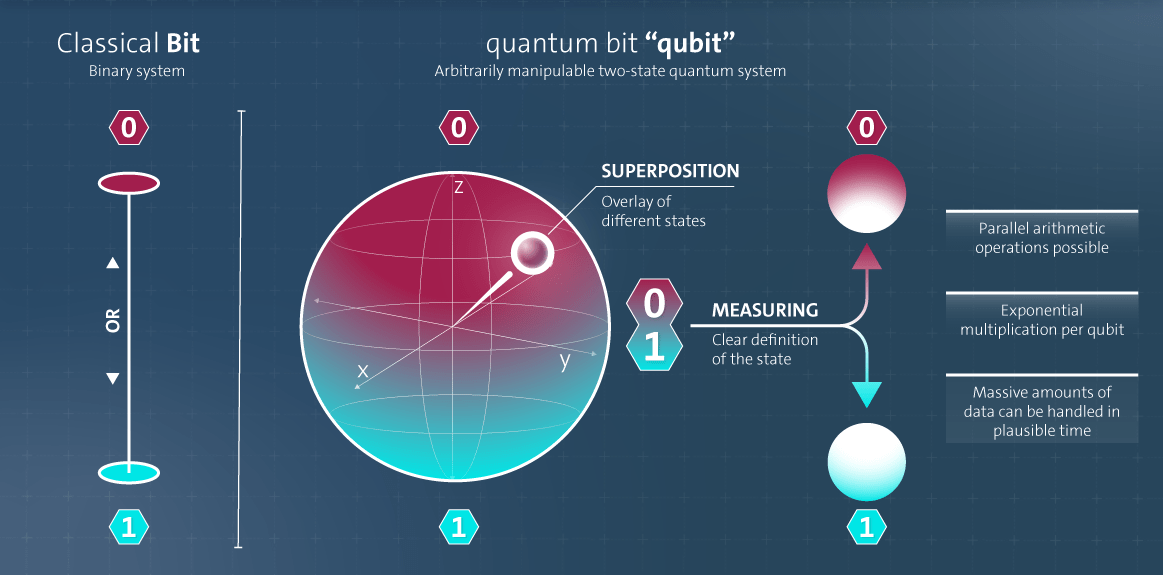
\includegraphics[width=11cm]{fig/bitQubit.png}
\end{center}

\end{frame}

\section{Quantum Gates}

\begin{frame}\frametitle{Pauli X Gate}
\begin{center}
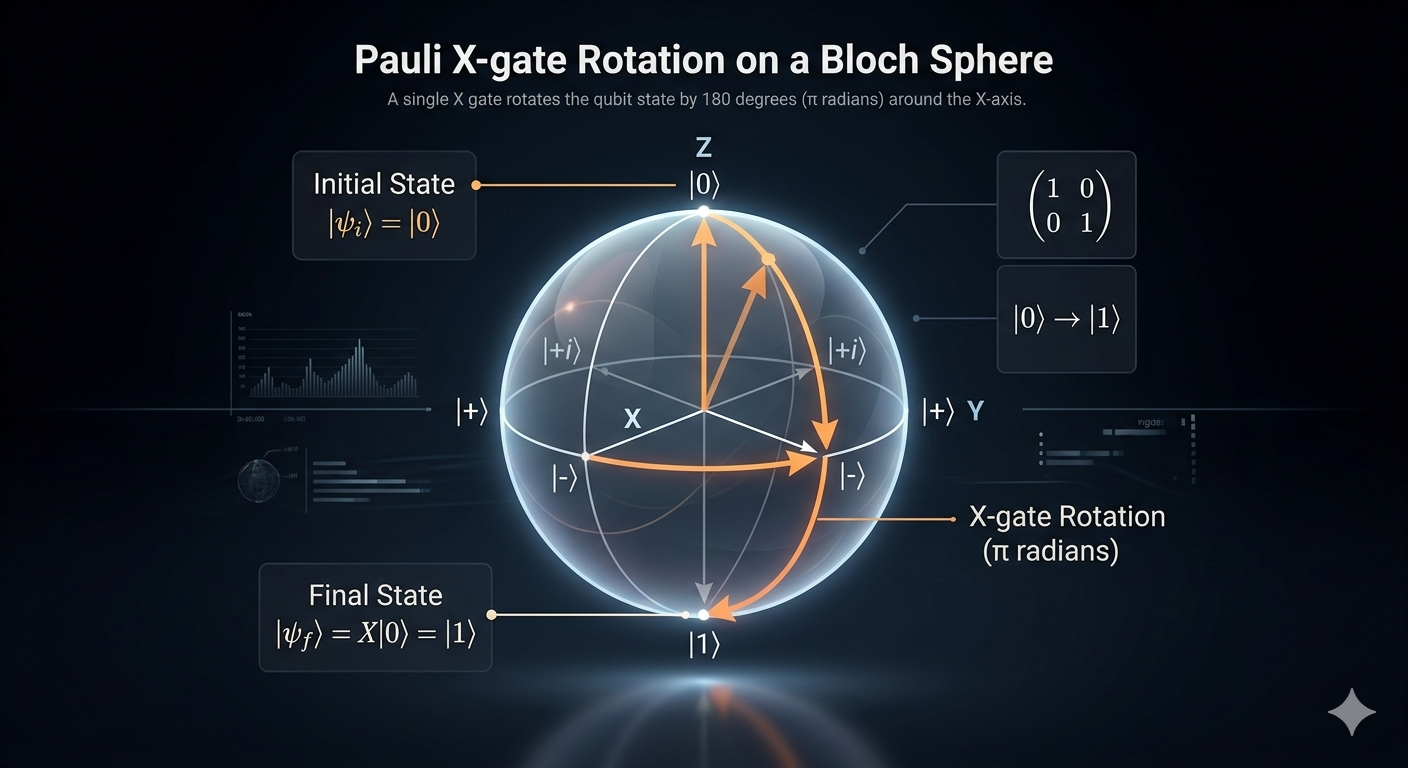
\includegraphics[width=12cm]{fig/GateX.png}
\end{center}
\end{frame}

\begin{frame}\frametitle{Pauli Y Gate}
\begin{center}
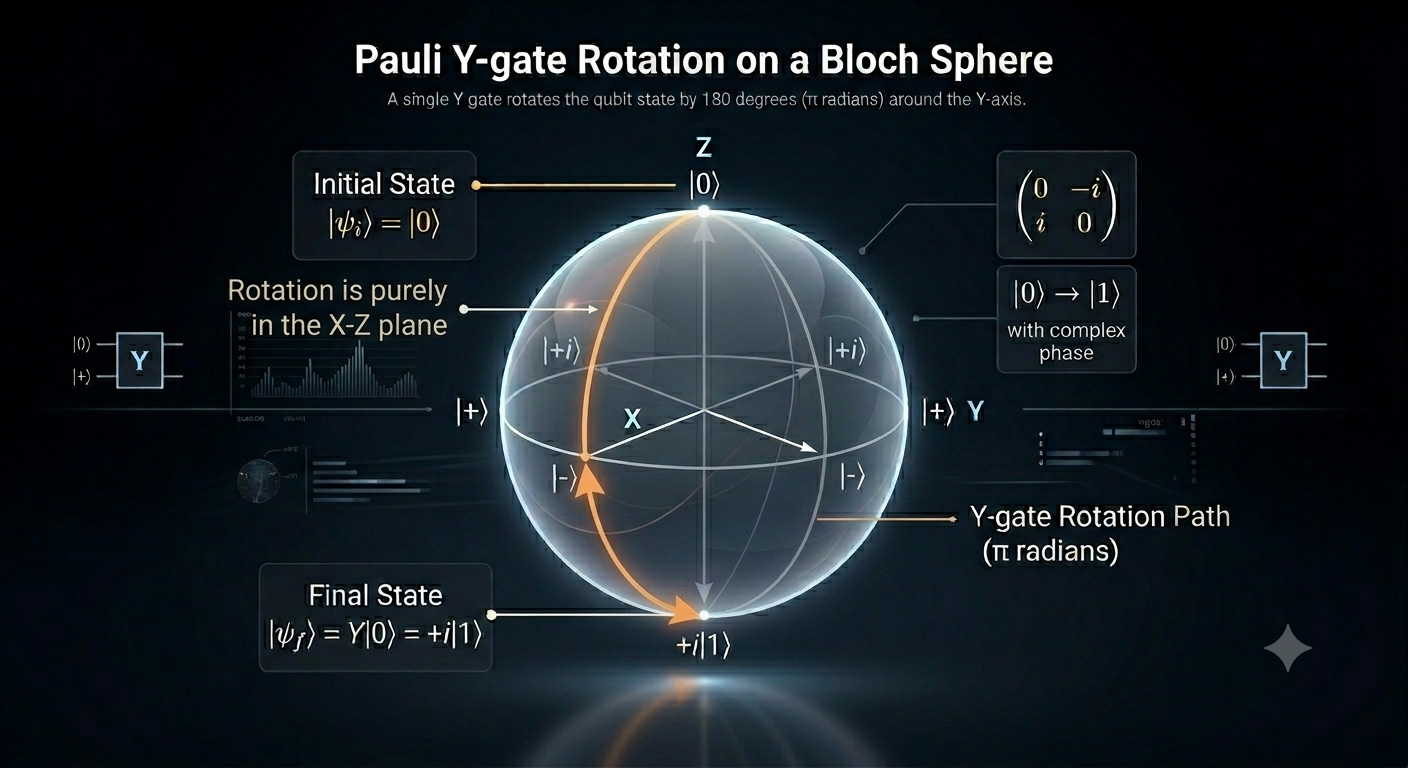
\includegraphics[width=12cm]{fig/GateY.png}
\end{center}
\end{frame}

\begin{frame}\frametitle{Pauli Z Gate}
\begin{center}
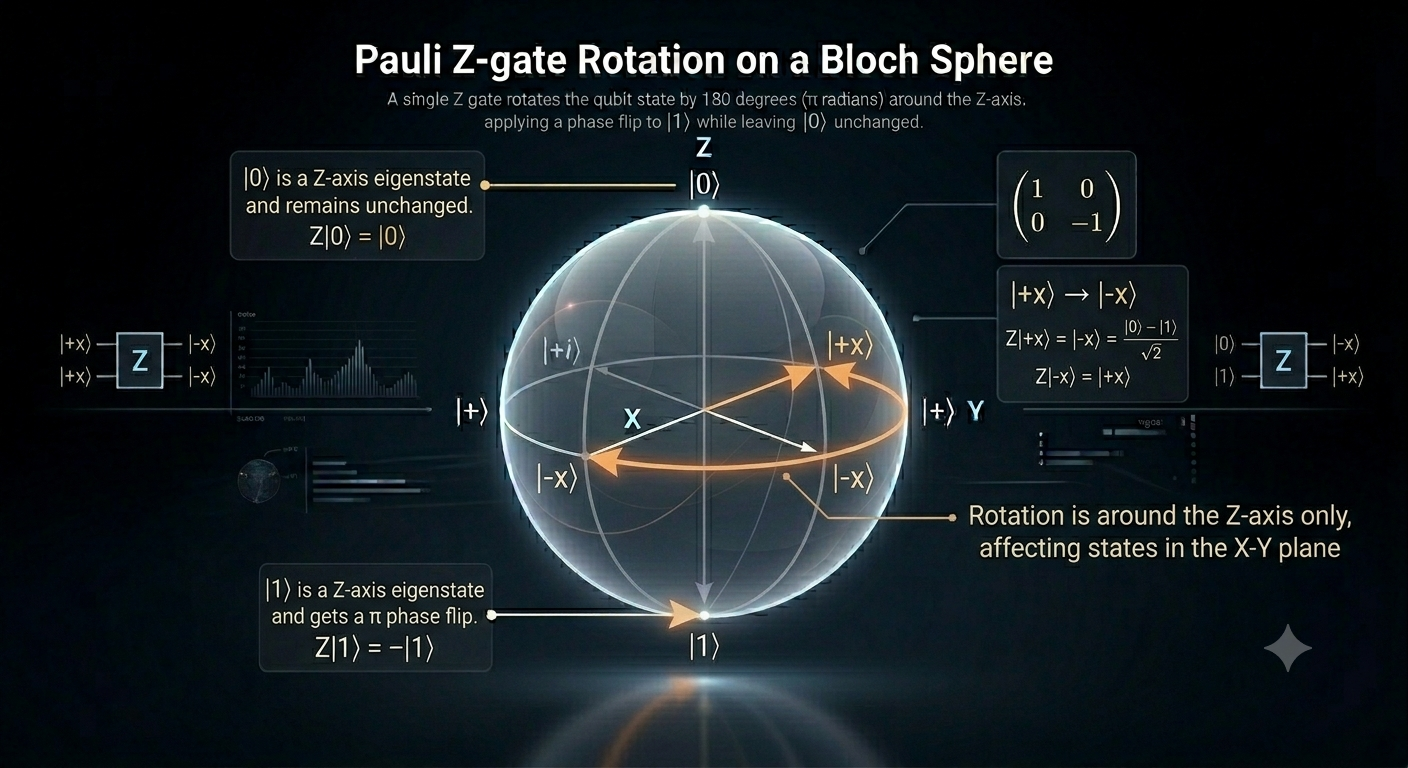
\includegraphics[width=12cm]{fig/GateZ.png}
\end{center}
\end{frame}

\begin{frame}\frametitle{Hadamond Gate}
\begin{center}
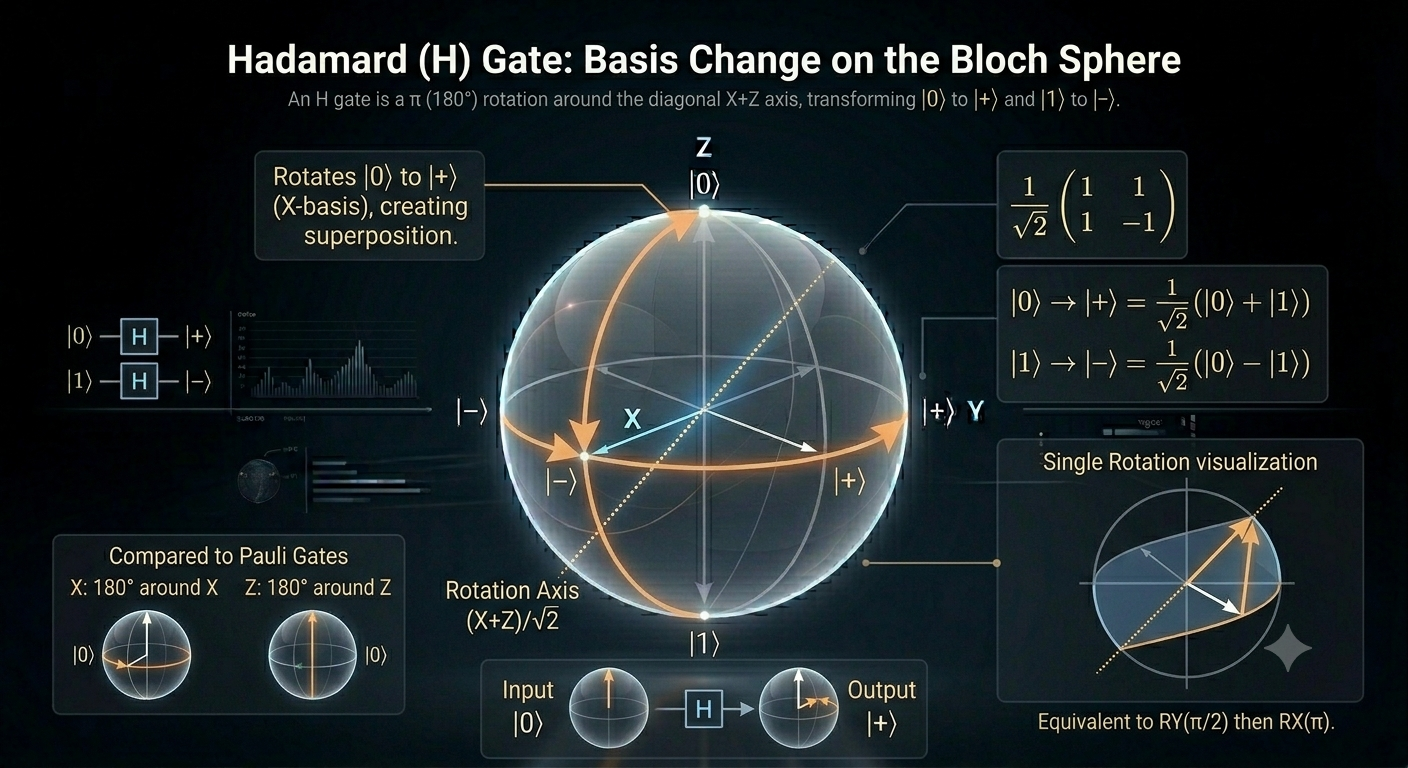
\includegraphics[width=12cm]{fig/GateH.png}
\end{center}
\end{frame}

\begin{frame}\frametitle{S Gate or Phase Gate}
\begin{center}
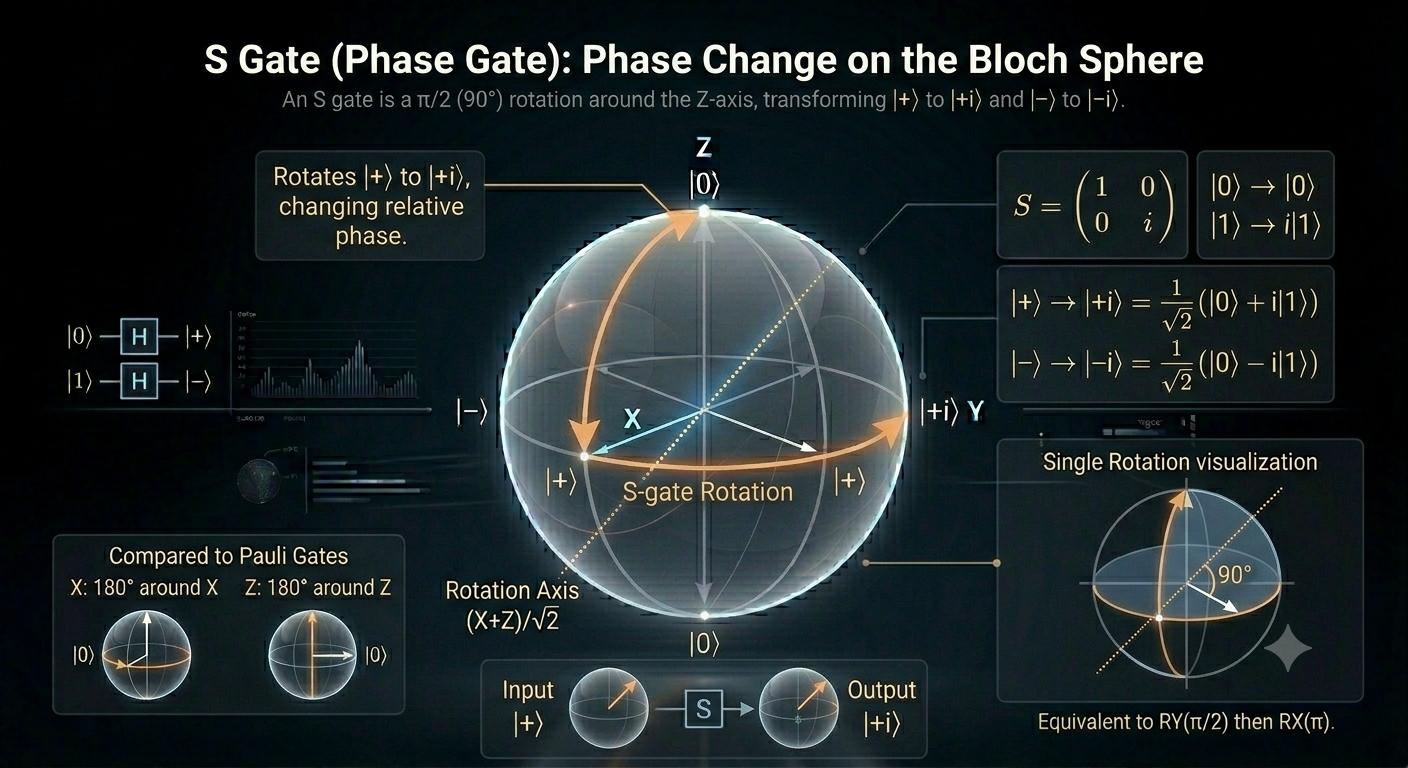
\includegraphics[width=12cm]{fig/GateS.png}
\end{center}
\end{frame}

\begin{frame}\frametitle{T Gate or $\frac{\pi}{8}$ Phase Gate}
\begin{center}
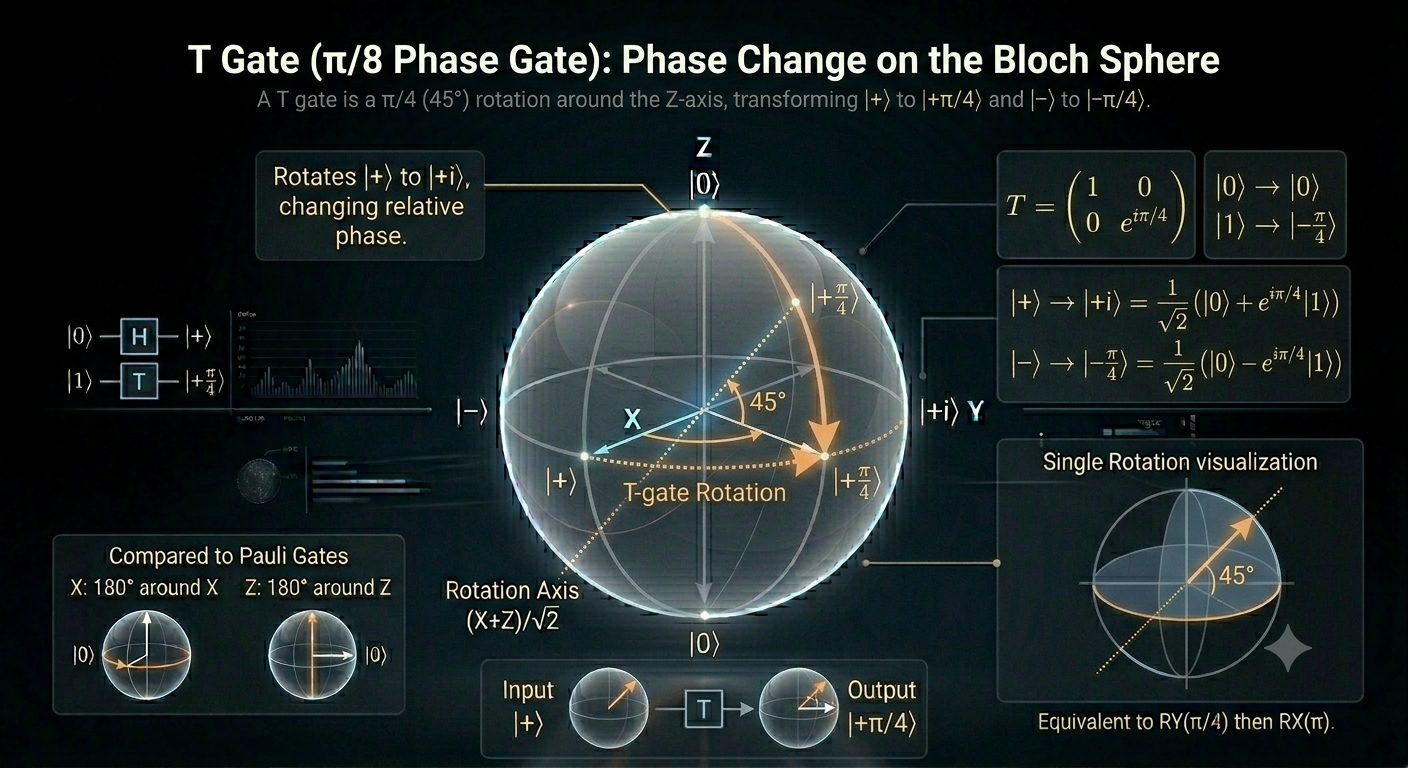
\includegraphics[width=12cm]{fig/GateT.png}
\end{center}
\end{frame}

\begin{frame}\frametitle{Anatomy of a Quantum Circuit}
\begin{center}
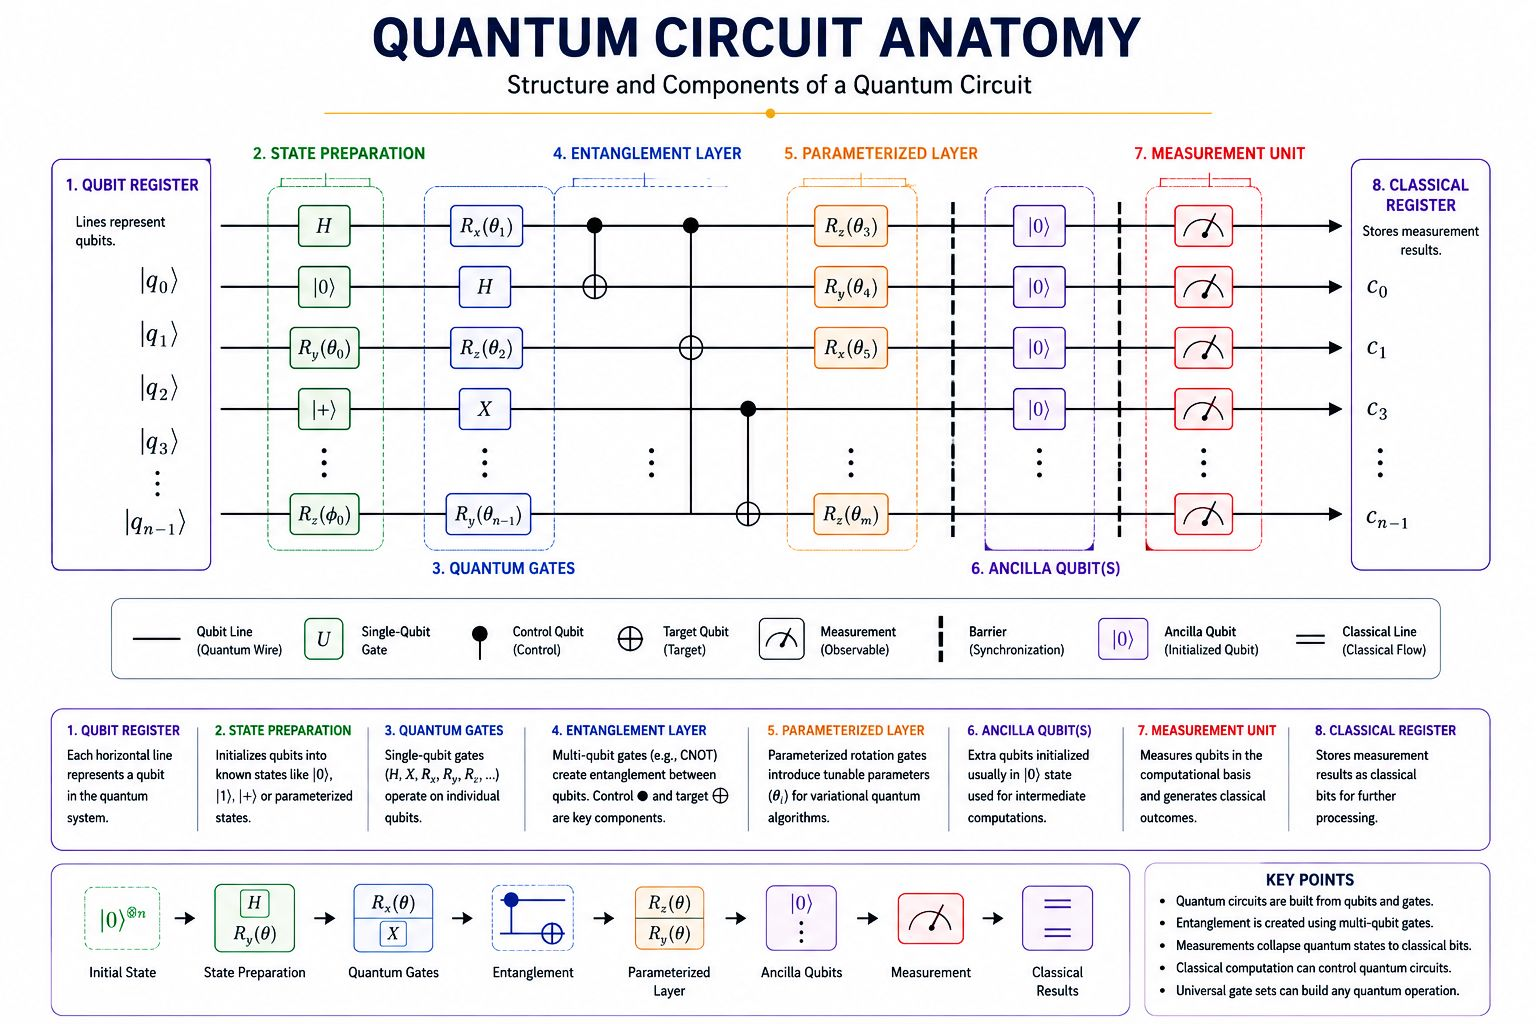
\includegraphics[width=11cm]{fig/qcircuit.jpg}
\end{center}
\end{frame}

\section{Quantum Computing}

\begin{frame}\frametitle{Types of Quantum Computers}
\begin{itemize}
\item Superconducting
\item Photonic
\item Neutral Atom
\item Trapped Ion
\item Quantum Dots
\item Diamond Nitrogen Vacancies
\end{itemize}
\end{frame}

\begin{frame}\frametitle{Natural vs Manmade}
\begin{center}
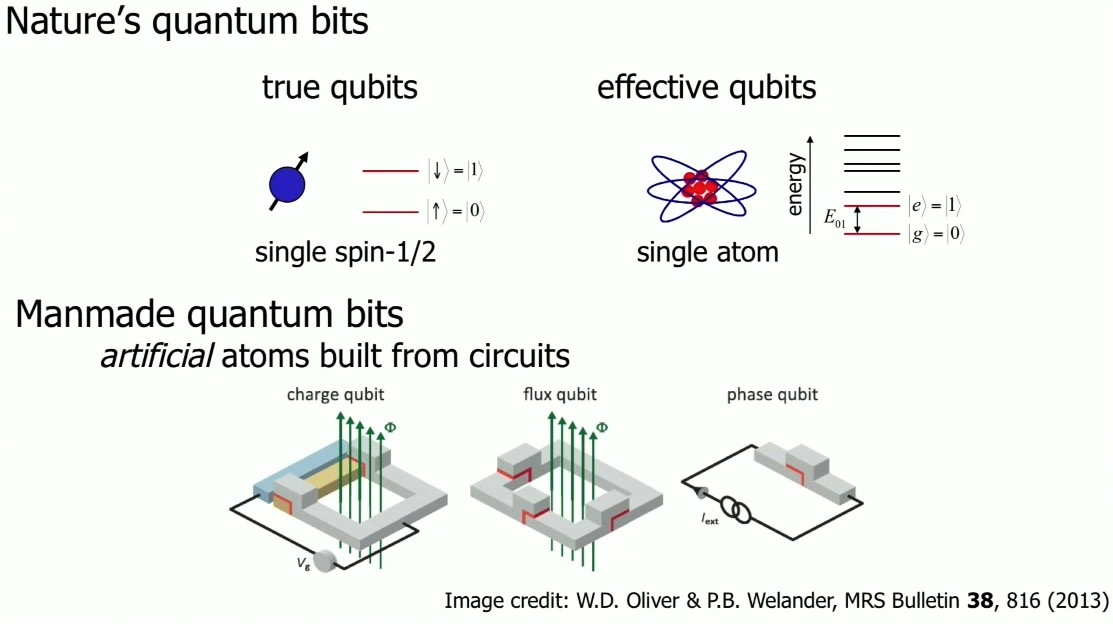
\includegraphics[width=11cm]{fig/typeofqubit0.jpg}
\end{center}
\end{frame}


\begin{frame}\frametitle{Quantum Computing: Superconducting}
One of the most popular types of quantum computers is a superconducting qubit quantum computer. Usually made from superconducting materials, these quantum computers utilize tiny electrical circuits to produce and manipulate qubits. When using superconducting qubits, gate operations can be performed quickly.

Companies actively researching and manufacturing superconducting quantum computers include Google, IBM, IQM and Rigetti Computing to name just a few.
\end{frame}

\begin{frame}\frametitle{Superconducting Explored: Transmon QuBit}
\begin{center}
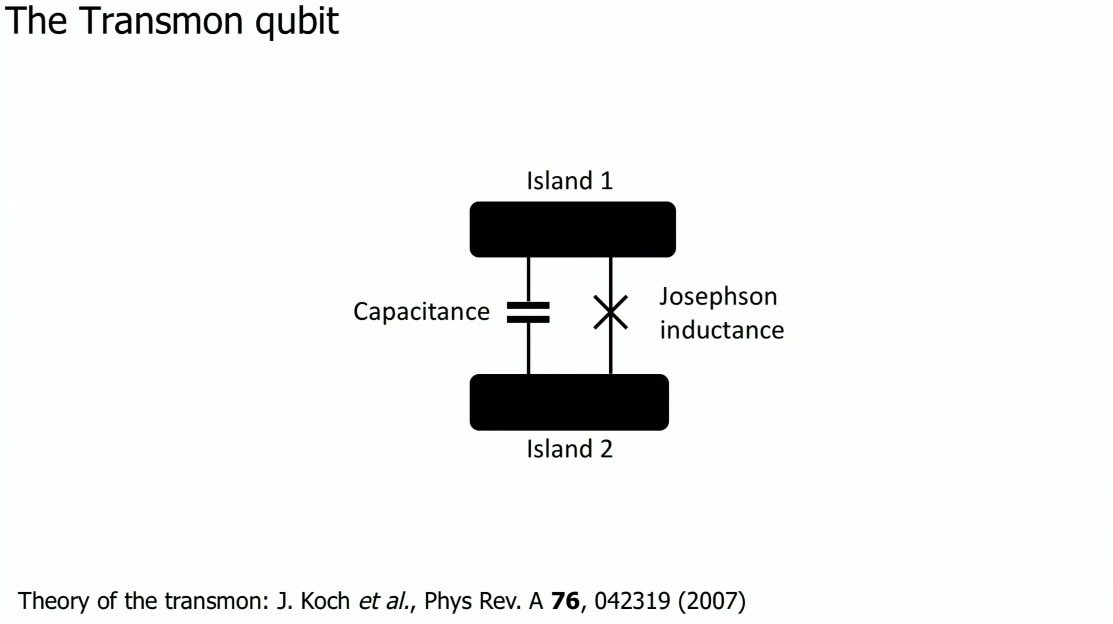
\includegraphics[width=12cm]{fig/typeofqubit1.jpg}
\end{center}
\end{frame}

\begin{frame}\frametitle{Superconducting Explored: LC Oscillator}
\begin{center}
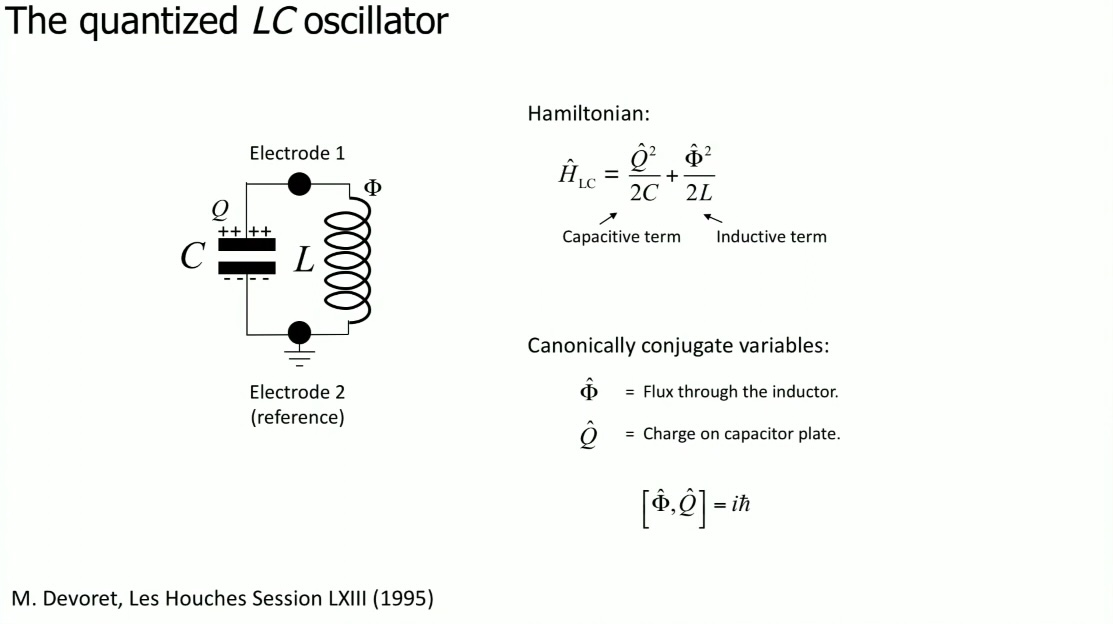
\includegraphics[width=12cm]{fig/typeofqubit2.jpg}
\end{center}
\end{frame}

\begin{frame}\frametitle{Superconducting Explored: Harmonic Oscillator}
\begin{center}
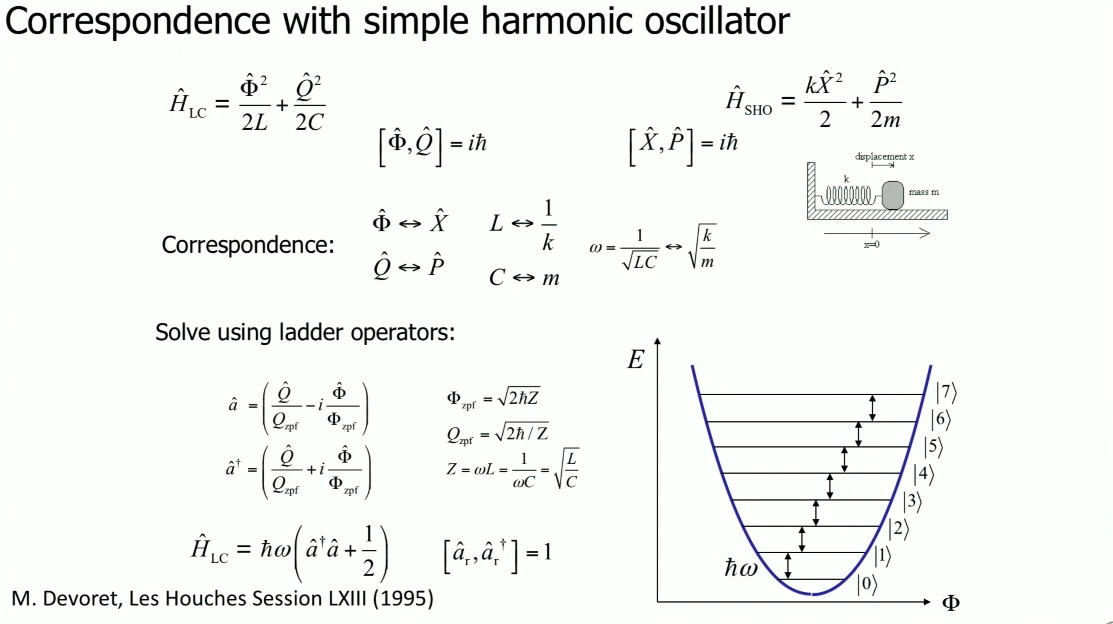
\includegraphics[width=12cm]{fig/typeofqubit3.jpg}
\end{center}
\end{frame}

\begin{frame}\frametitle{Superconducting Explored: Josephson Junction}
\begin{center}
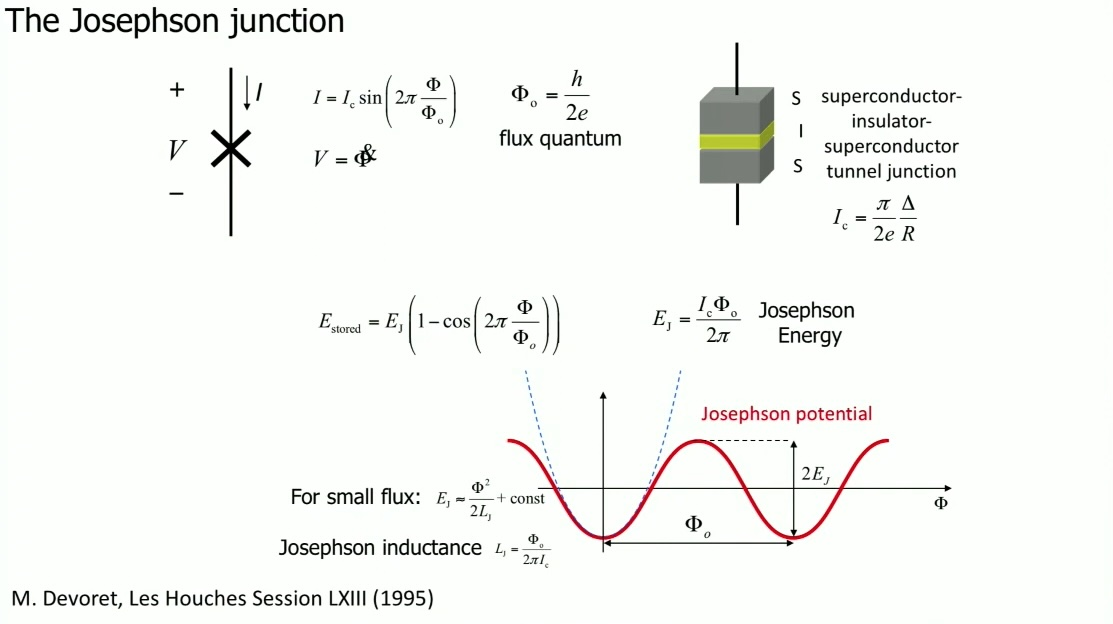
\includegraphics[width=12cm]{fig/typeofqubit4.jpg}
\end{center}
\end{frame}

\begin{frame}\frametitle{Superconducting Explored: Energy Quantization Spectrum}
\begin{center}
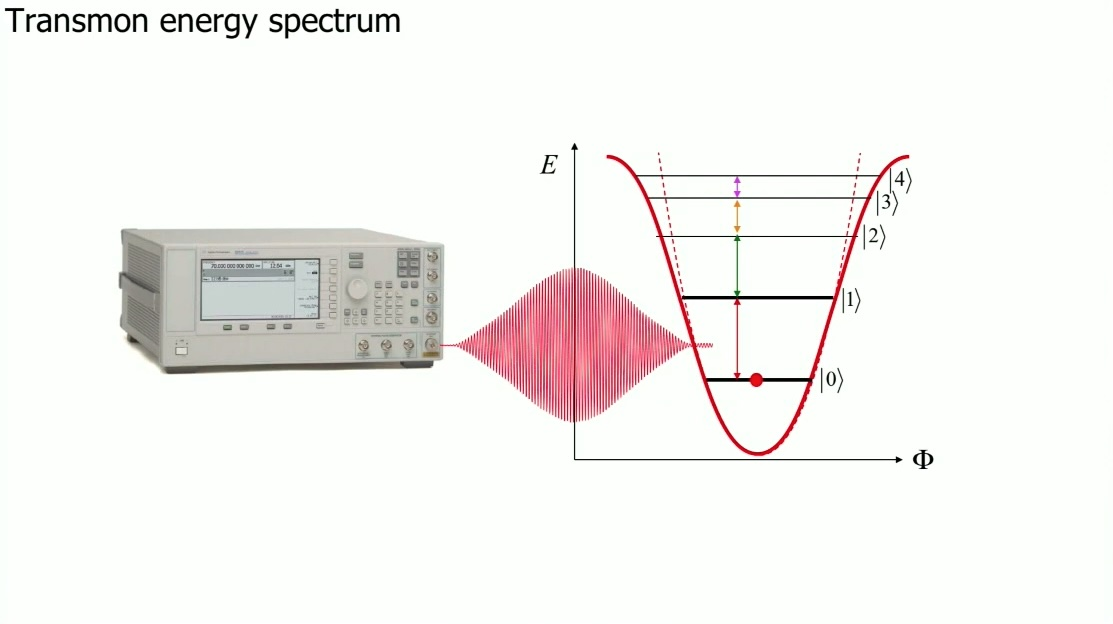
\includegraphics[width=12cm]{fig/typeofqubit5.jpg}
\end{center}
\end{frame}

\begin{frame}\frametitle{Superconducting Explored: Josephson Junction}
\begin{center}
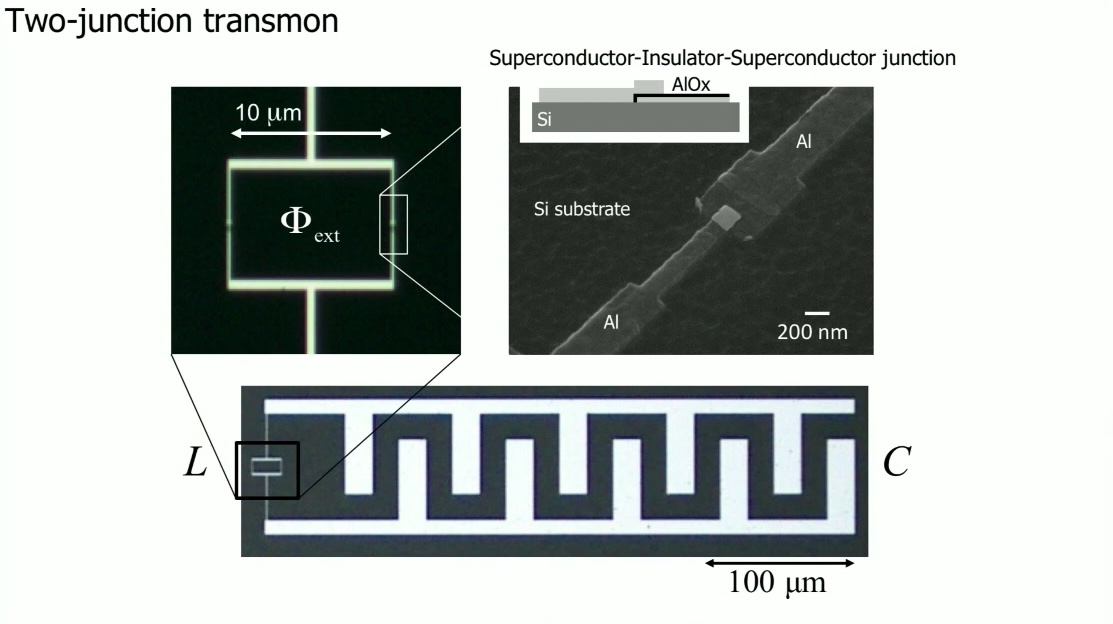
\includegraphics[width=12cm]{fig/typeofqubit6.jpg}
\end{center}
\end{frame}

\begin{frame}\frametitle{Superconducting Explored: QuBit Resonator}
\begin{center}
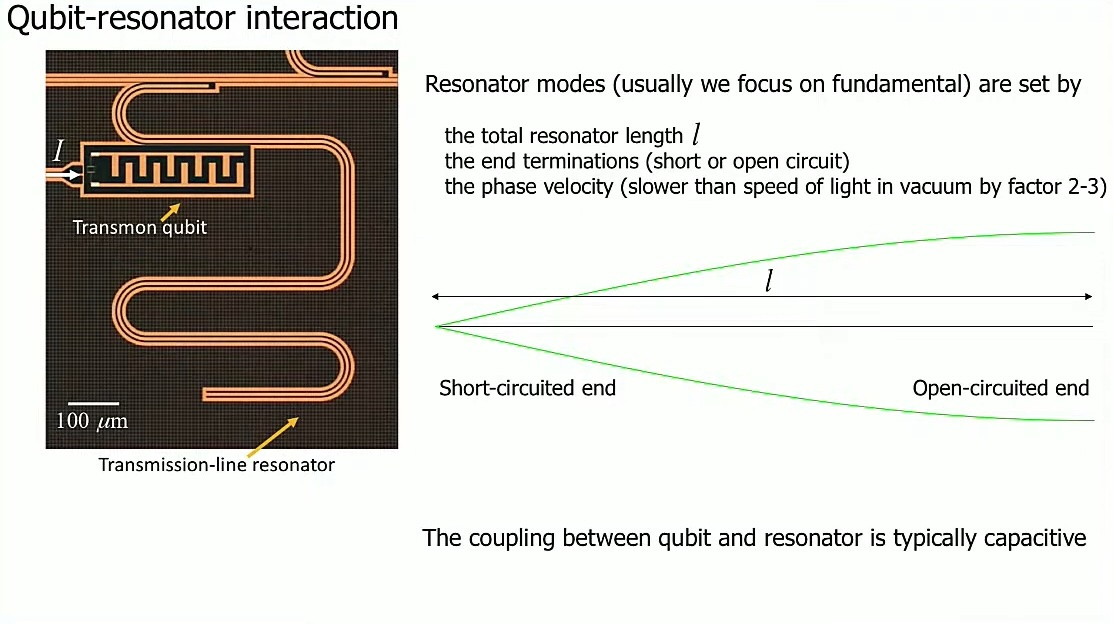
\includegraphics[width=12cm]{fig/typeofqubit7.jpg}
\end{center}
\end{frame}

\begin{frame}\frametitle{Superconducting Explored: Two QuBit}
\begin{center}
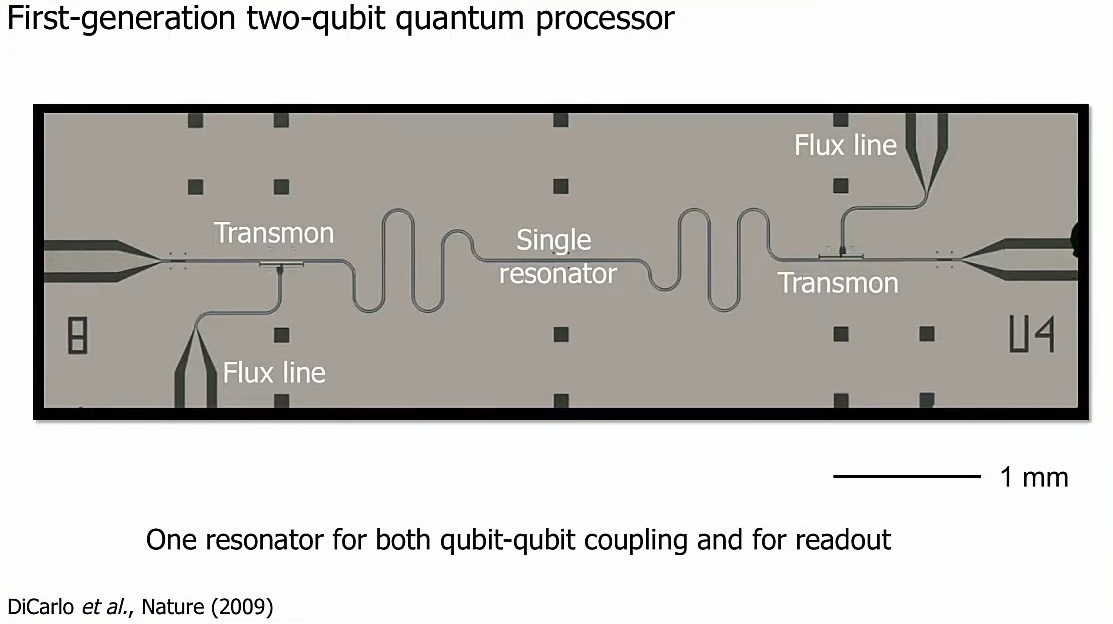
\includegraphics[width=12cm]{fig/typeofqubit8.jpg}
\end{center}
\end{frame}

\begin{frame}\frametitle{Superconducting Explored: Two QuBit Improved}
\begin{center}
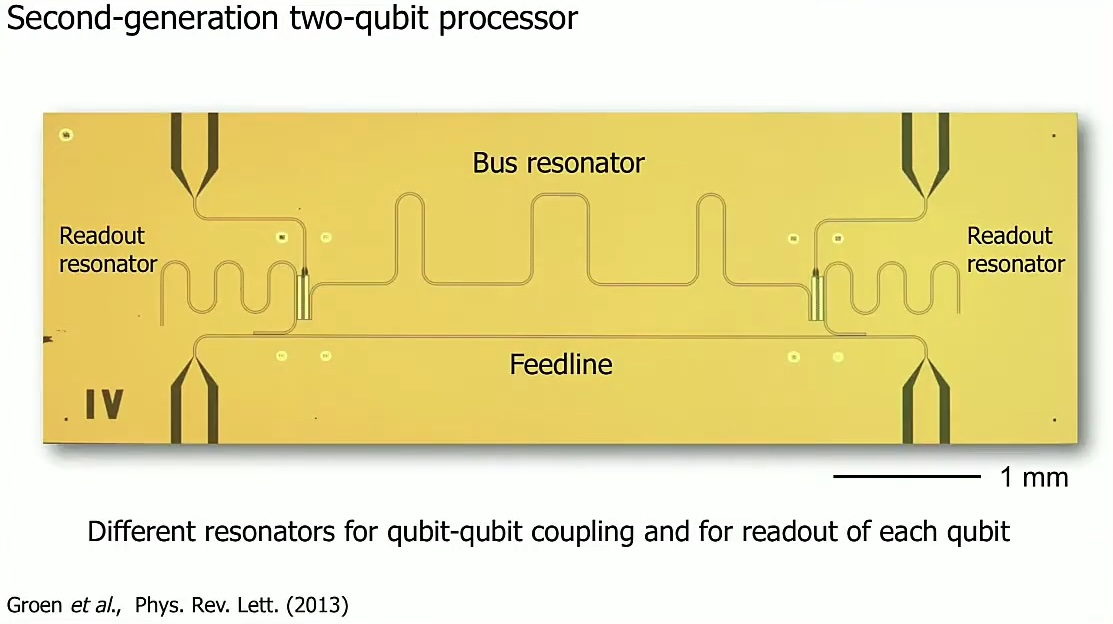
\includegraphics[width=12cm]{fig/typeofqubit9.jpg}
\end{center}
\end{frame}

\begin{frame}\frametitle{Superconducting Explored: Four QuBit}
\begin{center}
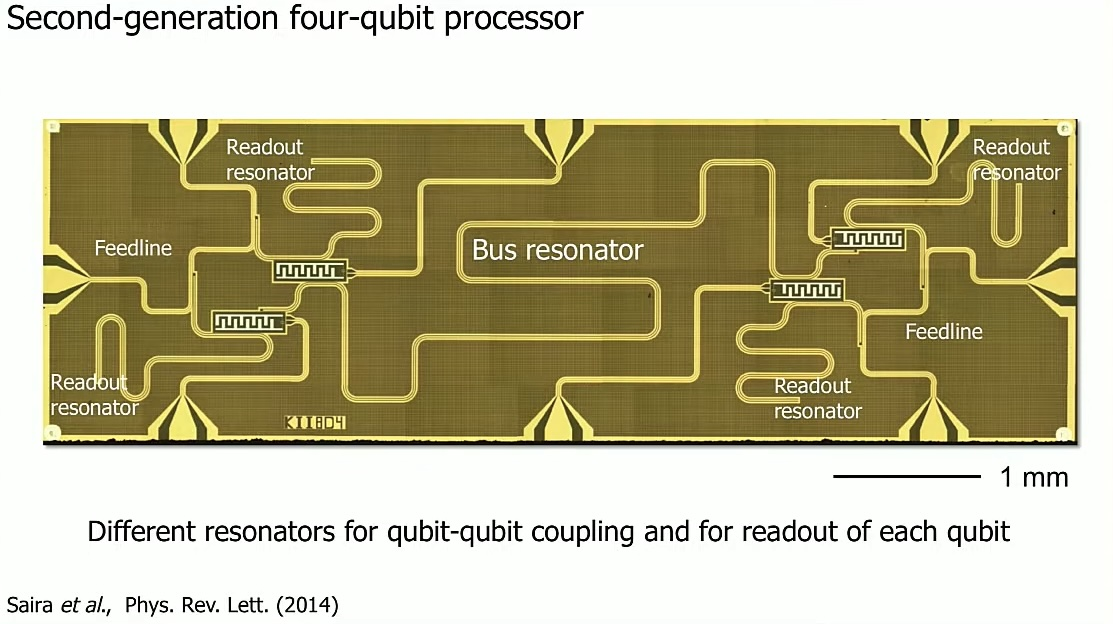
\includegraphics[width=12cm]{fig/typeofqubitA.jpg}
\end{center}
\end{frame}

\begin{frame}\frametitle{Superconducting Explored: Four QuBit}
\begin{center}
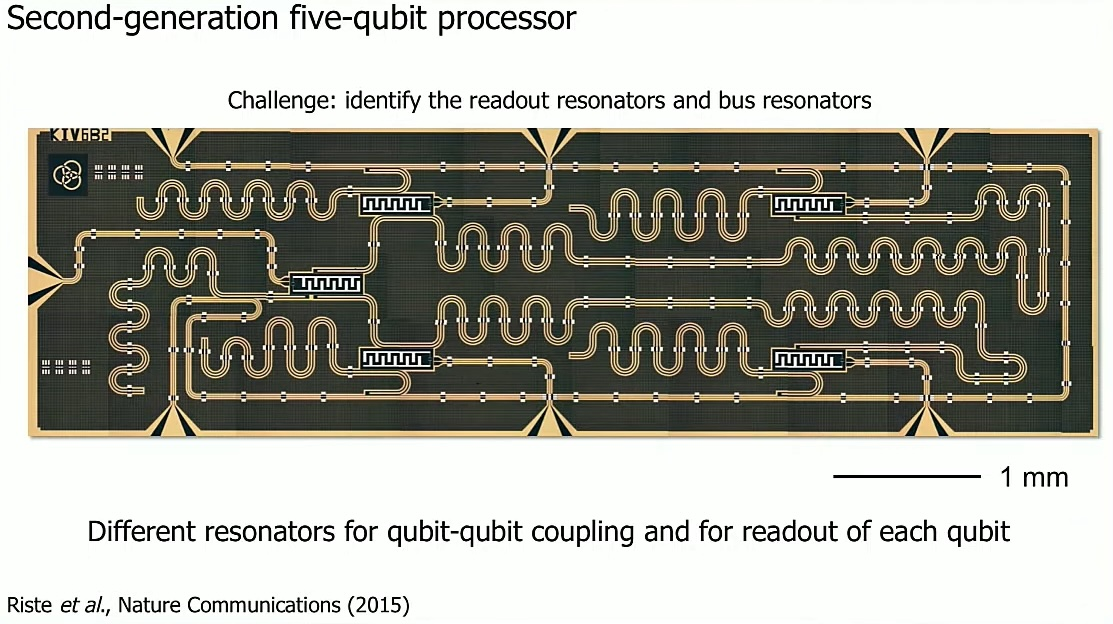
\includegraphics[width=12cm]{fig/typeofqubitB.jpg}
\end{center}
\end{frame}

\begin{frame}\frametitle{Superconducting Explored: Readout}
\begin{center}
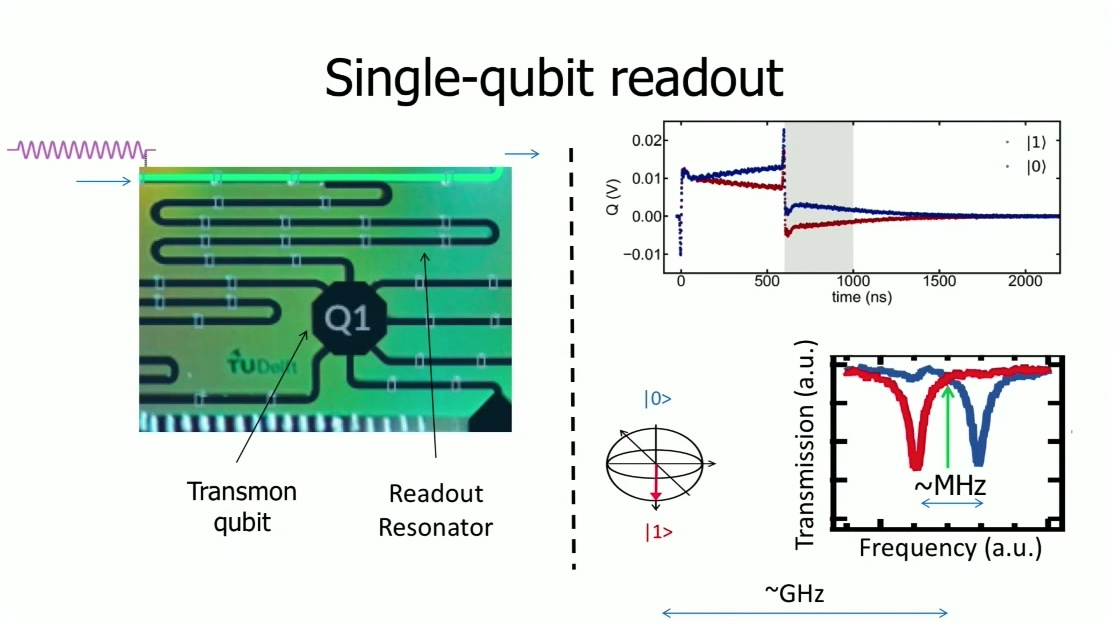
\includegraphics[width=12cm]{fig/typeofqubitD.jpg}
\end{center}
\end{frame}


\begin{frame}\frametitle{Superconducting Explored: Readout Noise}
\begin{center}
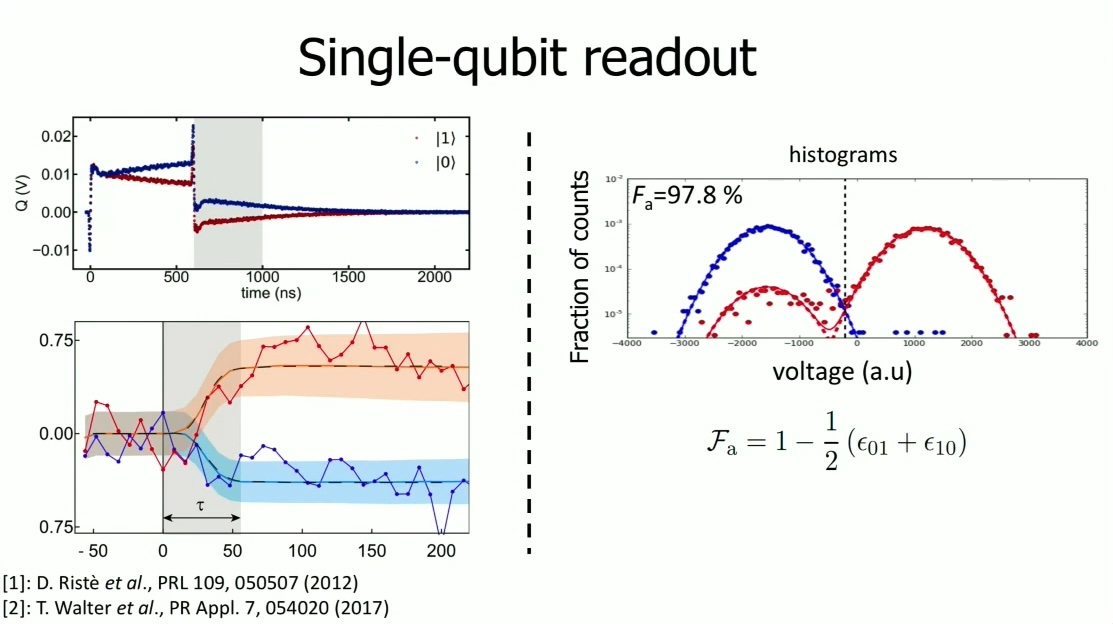
\includegraphics[width=12cm]{fig/typeofqubitE.jpg}
\end{center}
\end{frame}

\begin{frame}\frametitle{Superconducting Explored: Two QuBit Readout}
\begin{center}
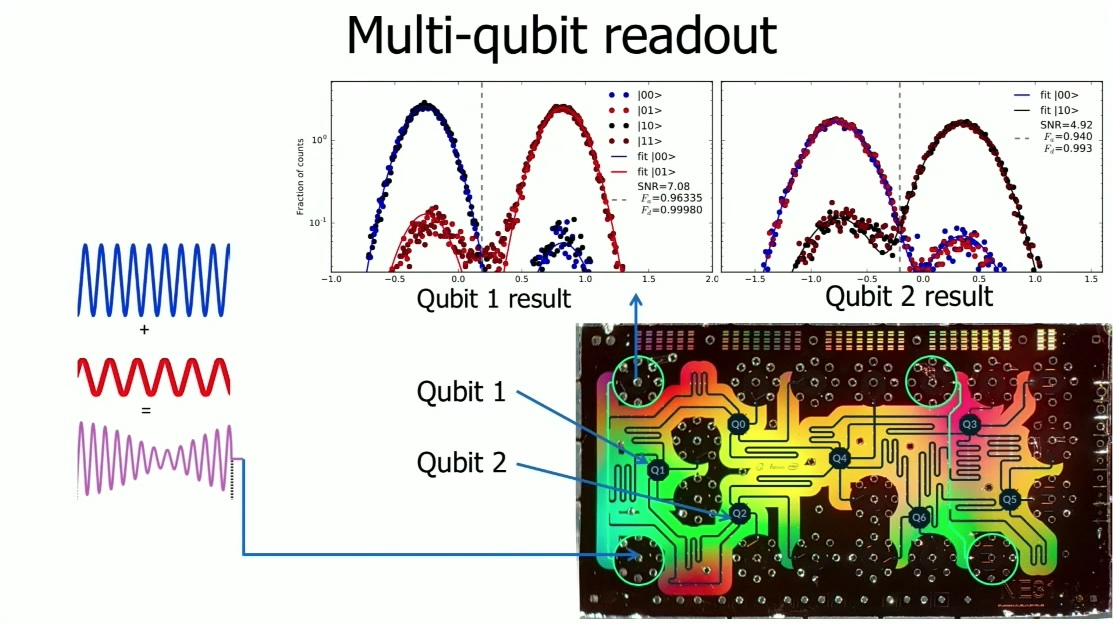
\includegraphics[width=12cm]{fig/typeofqubitF.jpg}
\end{center}
\end{frame}

\begin{frame}\frametitle{Quantum Computing: Photonics}
These types of quantum computers use photons (particles of light) to carry and process quantum information. For large-scale quantum computers, photonic qubits are a promising alternative to trapped ions and neutral atoms that require cryogenic or laser cooling.
\end{frame}


\begin{frame}\frametitle{Quantum Computing: Neutral Atom}
Quantum computing based on neutral atoms involves atoms suspended in an ultrahigh vacuum by arrays of tightly focused laser beams called optical tweezers, though not all neutral atom companies use optical tweezers. Neutral atom quantum computers are less sensitive to stray electric fields, which makes them a good option for quantum processors.
\end{frame}


\begin{frame} \frametitle{Trapped Ions}
\begin{center}
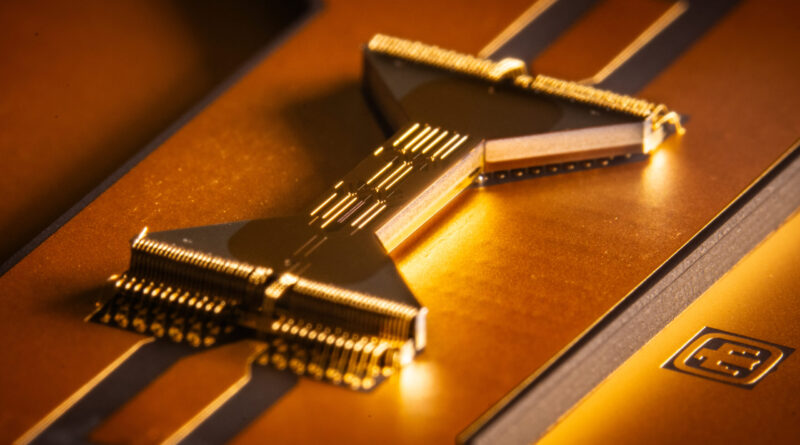
\includegraphics[width=5cm]{fig/qscoutTrappedIon.jpg}
\end{center}

A trapped ion quantum computer involves using atoms or molecules with a net electrical charge known as “ions” that are trapped and manipulated using electric and magnetic fields to store and process quantum information. As trapped ions can be isolated from their environment, they are useful for precision measurements and other applications requiring high levels of stability and control. Also, the qubits can remain in a superposition state for a long time before becoming decoherent.

Representing the trapped ions community of companies in the quantum space, we have Quantinuum (a company that came out of the merger between Cambridge Quantum Computing and Honeywell Quantum Solutions), IonQ, Quantum Factory, Alpine Quantum Technologies, eleQtron amongst others

\end{frame}


\begin{frame}\frametitle{Quantum Computing: Quantum Dots}
A quantum dot quantum computer uses silicon qubits made up of pairs of quantum dots. In theory for quantum computers, such ‘coupled’ quantum dots could be used as robust quantum bits, or qubits.

Companies focused on this area include Diraq, Siquance and Quantum Motion.
\end{frame}

\begin{frame}\frametitle{Quantum Computing: NV Diamond}
\begin{center}
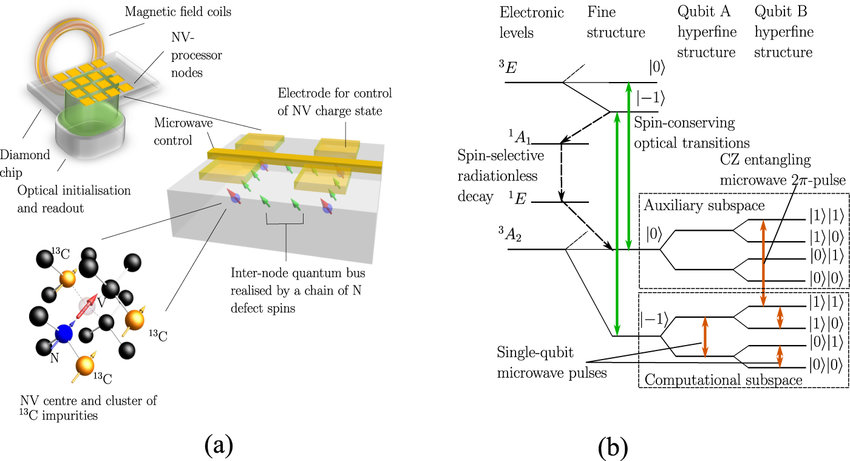
\includegraphics[width=12cm]{fig/nvCompute.png}
\end{center}
\end{frame}

\section{Quantum Teleportation}

\begin{frame}\frametitle{Practice Frame}

These commands write quantum-mechanical bras and kets, such as \bra{\alpha} and \ket{\beta}, as well as their products, like \bracket{\alpha}{\eta}, and also matrix elements such as \matrixel{\xi}{T}{\pi}. They're quite useful when one of the factors is large: for instance \ket{\xi} vs \ket{\hat{\xi}}, or when one has \matrixel{\xi}{\hat{T}}{\pi}.

There's only one funny space, in the bracket (as opposed to the ket) below, which shouldn't really be there, and which I can't really figure out:
\begin{align*}
a\ket{\alpha,1}&=\alpha\ket{\alpha,1}+\ket{\alpha}\\
\bracket{\alpha,1}{\alpha,1}&=1
\end{align*}

\[ \ket{\psi} = \begin{pmatrix} c_{00} \\ c_{01} \\ c_{10} \\ c_{11} \end{pmatrix}\]


\end{frame}

\begin{frame}\frametitle{Teleportation Setup}
\begin{columns}
\begin{column}{5cm}
Alice has a qubit ($q_0$) whose state she wants to be able to send to Bob. Bob has two entangled qubits ($q_1$ and $q_2$), he gives $q_1$ to Alice. \newline

The entangled qubits are in a Bell State of $\beta_{00}$:
\[ \beta_{00} = \frac{1}{\sqrt{2}} (\ket{00} + \ket{11}) \]

The entire system is therefore in a state:
\[ \ket{\psi_0} = \ket{\psi} \ket{\beta_{00}} \]

\end{column}
\begin{column}{5.5cm}
\begin{center}
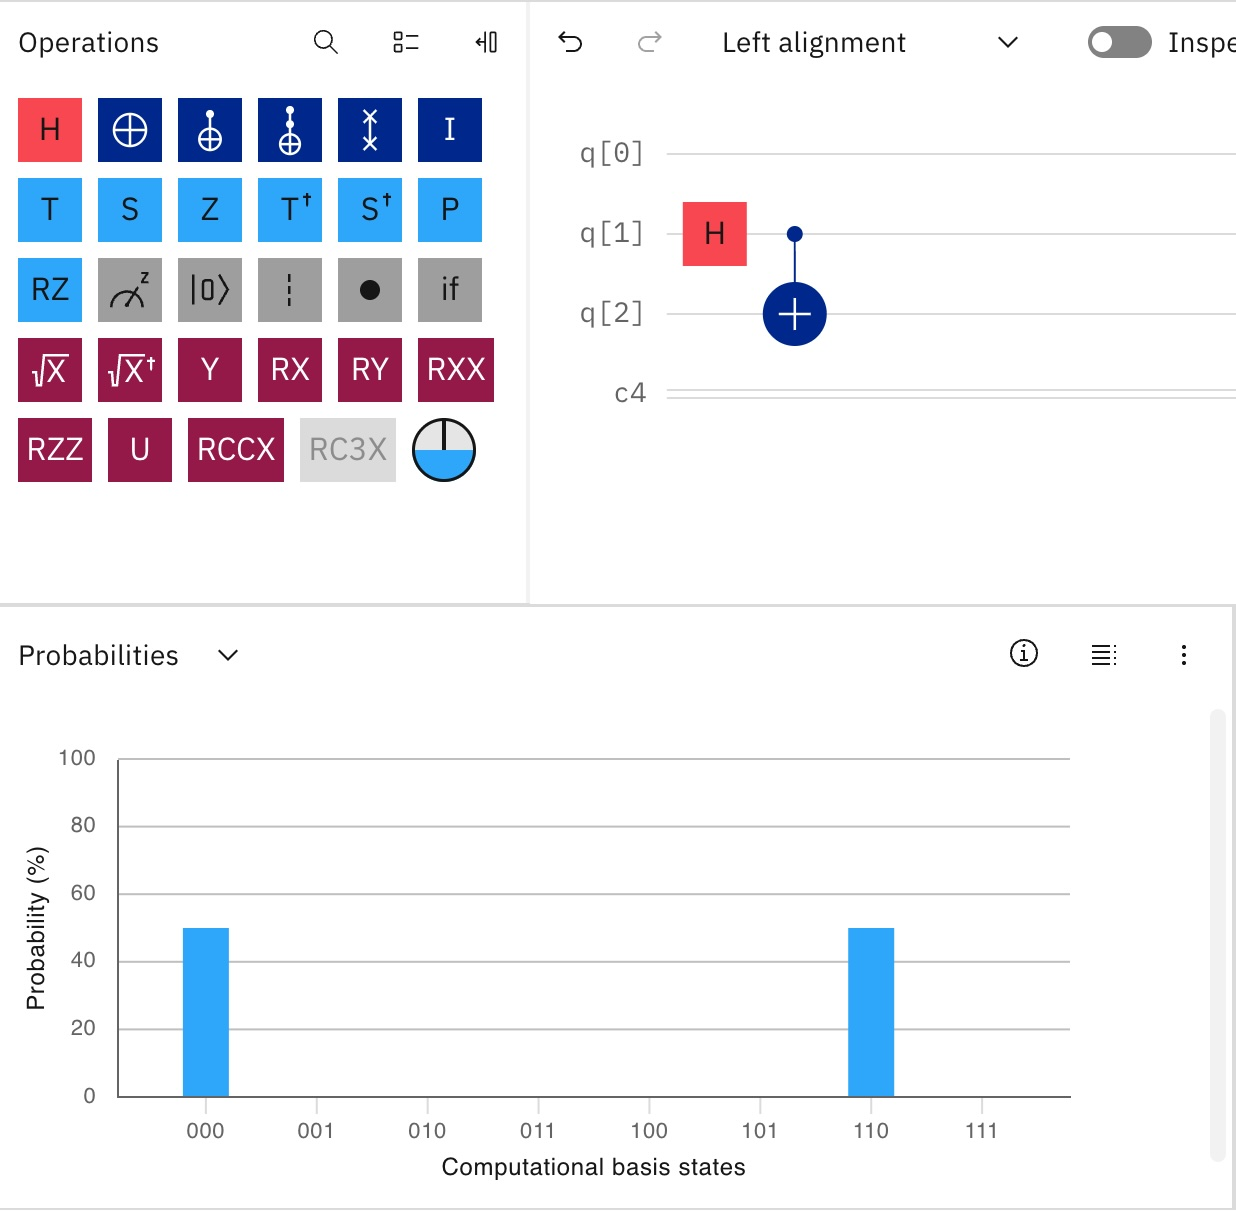
\includegraphics[width=5cm]{fig/qt1.jpg}
\end{center}
\end{column}
\end{columns}

\end{frame} 

\begin{frame}\frametitle{Initial State}

Expanding out the initial state:

\begin{align*}
\ket{\psi_0} &= \ket{\psi} \ket{\beta_{00}} \\
	&= (\alpha\ket{0} + \beta\ket{1}) (\frac{1}{\sqrt{2}} (\ket{00} + \ket{11})) \\
	&= \frac{1}{\sqrt{2}} \left[(\alpha\ket{0} (\ket{00} + \ket{11}) + (\beta\ket{1} (\ket{00} + \ket{11})\right]
\end{align*}

By convention, we consider the first two qubits belonging to alice
\end{frame}


\begin{frame}\frametitle{CNOT + Hadamond Math}
We next apply a CNOT gate to $q_1$ controlled by $q_0$:

\[ \ket{\psi_1} = \frac{1}{\sqrt{2}} \left[(\alpha\ket{0} (\ket{00} + \ket{11}) + (\beta\ket{1} (\ket{10} + \ket{01})\right] \]

Followed by a Hadamond Gate
\begin{itemize}
\item $H\ket{0} = \frac{\ket{0} + \ket{1}}{\sqrt{2}}$
\item $H\ket{1} = \frac{\ket{0} - \ket{1}}{\sqrt{2}}$
\end{itemize}

This results in:
\begin{align*}
\ket{\psi_2} =& \frac{1}{2} [\alpha (\ket{0} + \ket{1})(\ket{00} + \ket{11}) + 
							\beta (\ket{0} +-\ket{1})(\ket{10} + \ket{01})]
\end{align*}

\end{frame}

\begin{frame}\frametitle{CNOT + Hadamond Graphically}
\begin{center}
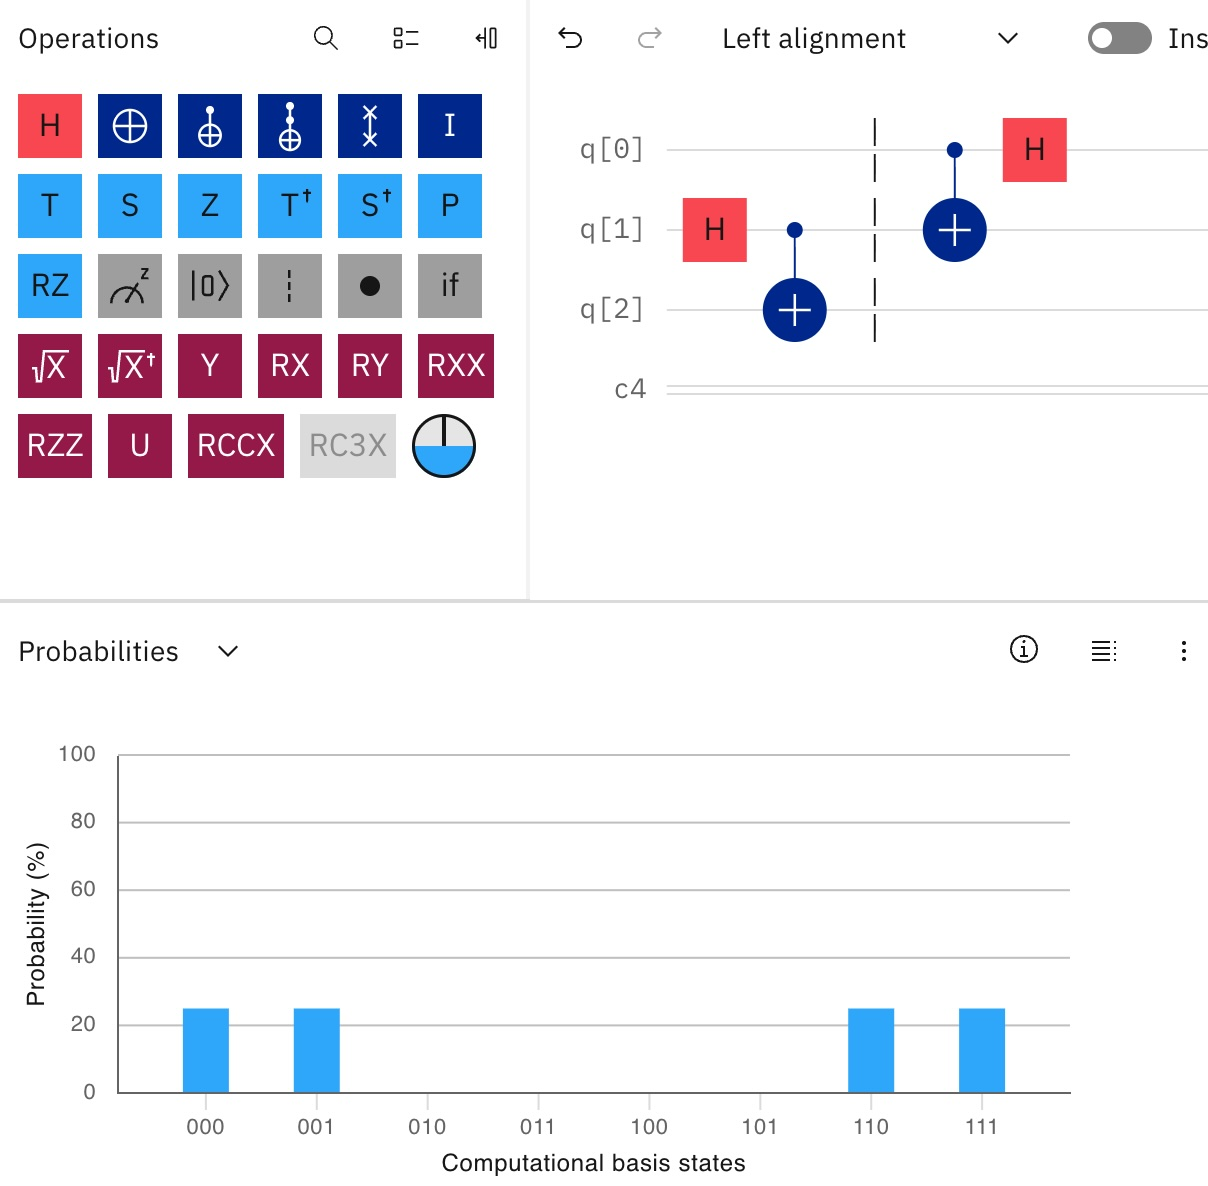
\includegraphics[width=7cm]{fig/qt2.jpg}
\end{center}
\end{frame}

\begin{frame}\frametitle{By Regrouping terms...}
Using the associative property:
\begin{align*}
\ket{\psi_2} =& \frac{1}{2} [ \ket{00}(\alpha\ket{0}+ \beta\ket{1}) +
									 \ket{01}(\alpha\ket{1}+ \beta\ket{0}) + \\
								 	&\ket{10}(\alpha\ket{0}- \beta\ket{1}) +
									 \ket{11}(\alpha\ket{1}- \beta\ket{0}) ]
\end{align*}

The first belong to Alice and the one in parenthesis belong to Bob. If Alice measures her qubits, there are four possibilities: 

\[00 \rightarrow \ket{\psi_3(00)} \equiv \alpha \ket{0} + \beta \ket{1}  \]
\[01 \rightarrow \ket{\psi_3(01)} \equiv \alpha \ket{1} + \beta \ket{0}  \]
\[10 \rightarrow \ket{\psi_3(10)} \equiv \alpha \ket{0} - \beta \ket{1}  \]
\[11 \rightarrow \ket{\psi_3(11)} \equiv \alpha \ket{1} - \beta \ket{0}  \]
\end{frame}

\begin{frame}\frametitle{Alice Measures, Bob then ...}

We want Bob's qubit to match $\psi_0 = \alpha \ket{0} + \beta \ket(1)$. Alice measures here two qubits and classically sends her two results to Bob classically. Bob them applies the following gates:

\begin{itemize}
\item $00 \rightarrow \ket{\psi_3(00)} \equiv \alpha \ket{0} + \beta \ket{1} \rightarrow$ Bob does nothing
\item $01 \rightarrow \ket{\psi_3(01)} \equiv \alpha \ket{1} + \beta \ket{0} \rightarrow$ Bob applies Pauli-X gate
\item $10 \rightarrow \ket{\psi_3(10)} \equiv \alpha \ket{0} - \beta \ket{1} \rightarrow$ Bob applies Pauli-Z gate
\item $11 \rightarrow \ket{\psi_3(11)} \equiv \alpha \ket{1} - \beta \ket{0} \rightarrow$ Bob applies Pauli-X and Pauli-Z.
\end{itemize}

Bob now has a qubit that matches Alice's original $\ket{\psi_0}$ and he can be extremely far away from Alice when she does her measurements. This leads to the following two questions: 
\begin{itemize}
\item Did this violate the no cloning theorem?
\item Did this violate relativity, information can't be transmitted faster than the speed of light?
\end{itemize}



\end{frame}


\begin{frame}\frametitle{Quantum Teleportation}
\begin{center}
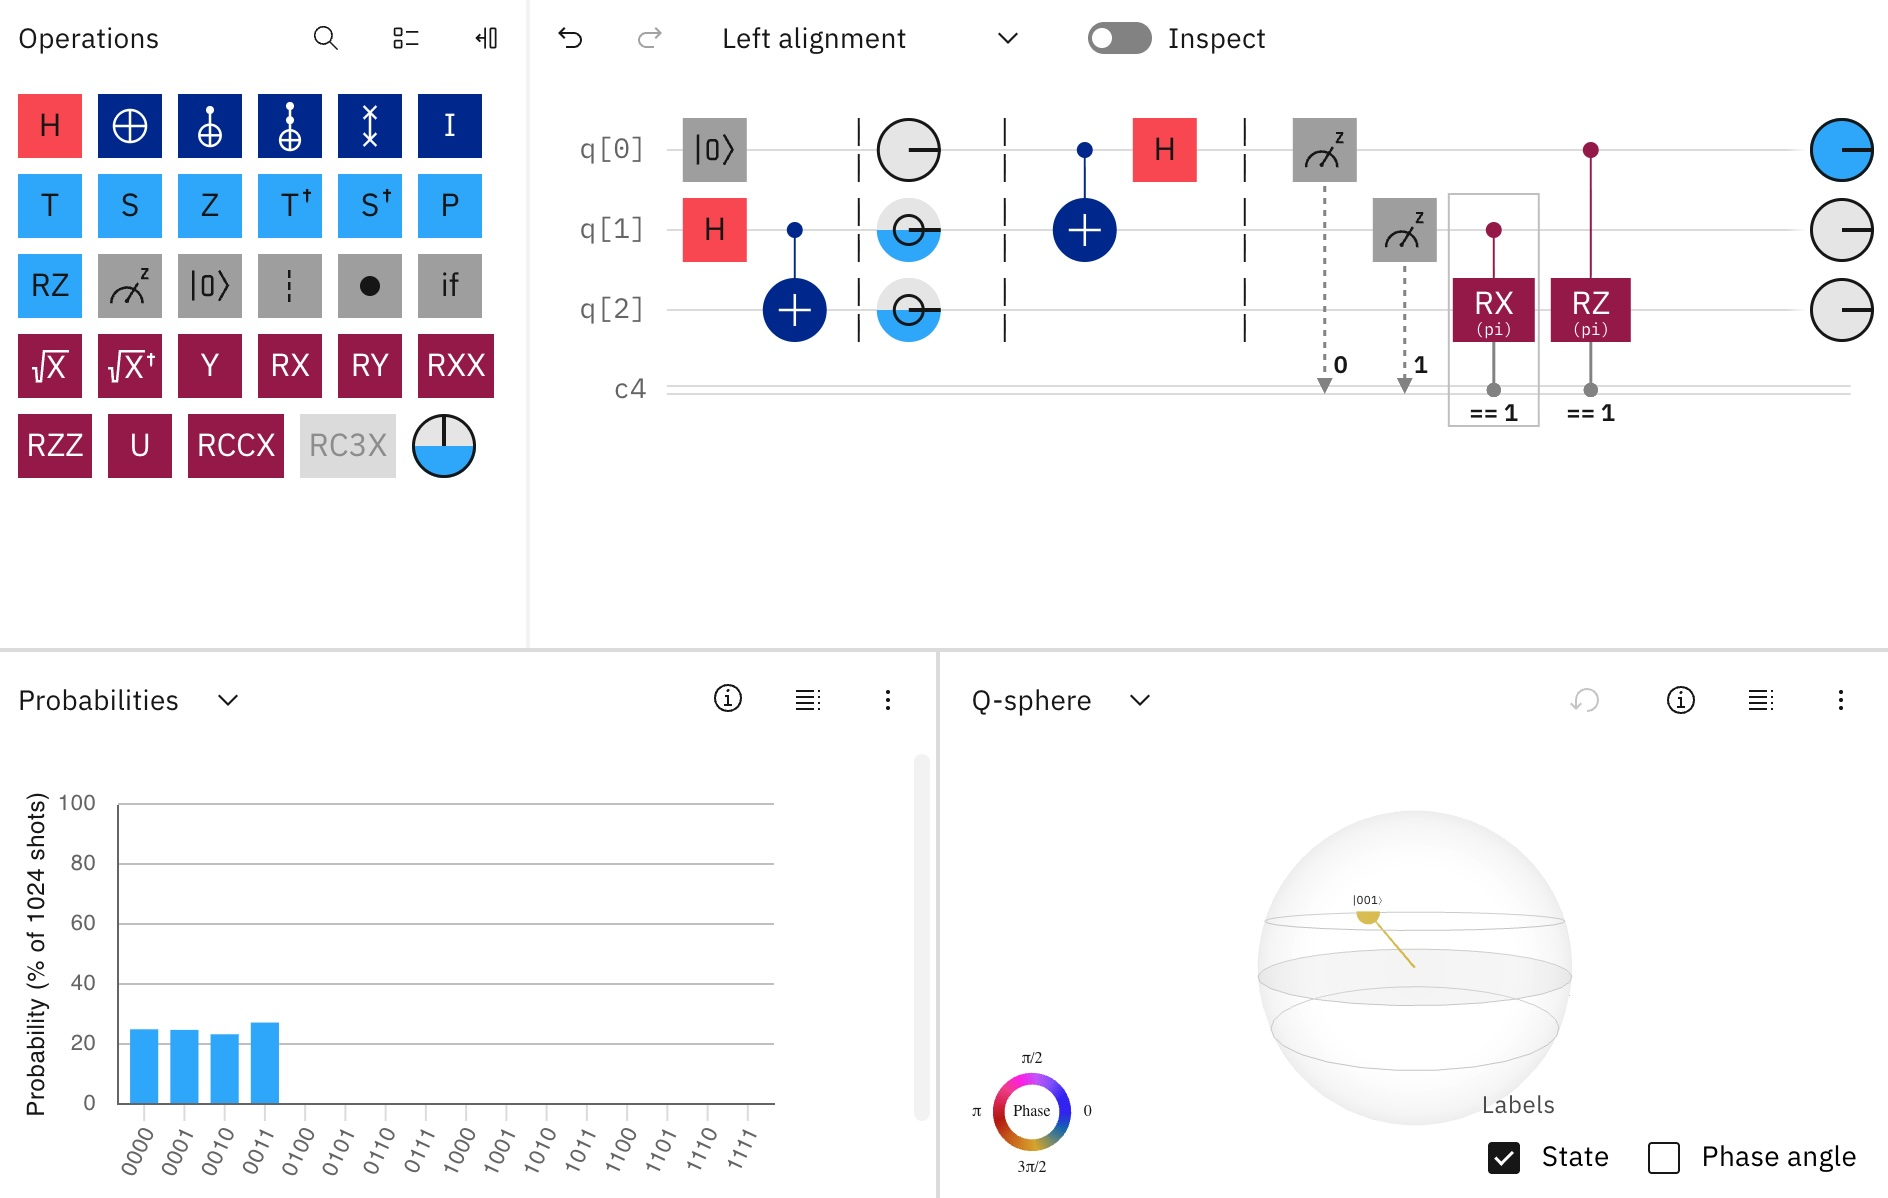
\includegraphics[width=11cm]{fig/qtdone.jpg}
\end{center}
\end{frame}

\end{document}
